\documentclass{standalone}
\usepackage{tikz}


\begin{document}

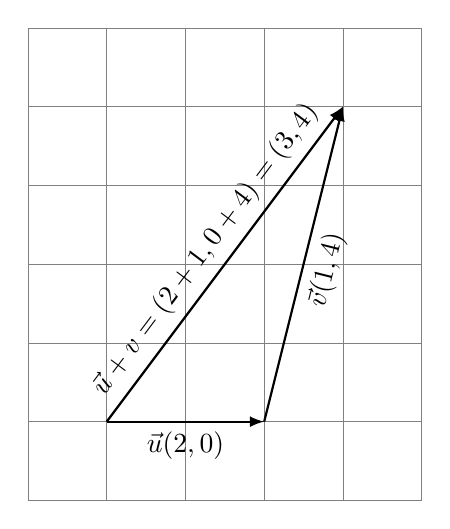
\begin{tikzpicture}
  \draw[help lines] (0,0) grid (5,6);

  \coordinate (p1) at (1,1);
  \coordinate (p2) at (3,1);
  \coordinate (p3) at (4,5);

  \draw[thick,-latex] (p1) -- (p2) node[below,midway] {$\vec u(2,0)$};
  \draw[thick,-latex] (p2) -- (p3) node[below,sloped,midway] {$\vec v(1,4)$};
  \draw[thick,-latex] (p1) -- (p3) node[above,sloped,midway] {$\vec u + v = (2+1, 0+4) = (3,4)$};
\end{tikzpicture}

\end{document}